% =====================================================================
%  Graph-Structured Reinforcement Learning for Fair and Efficient
%  CPU Process Scheduling
%
%  Humanized via HumanizeAI.pro (23 chunks processed).
%  Citations, equations, tables, and figures restored from original LaTeX.
%  Compiler: pdfLaTeX (Overleaf default) + BibTeX.
% =====================================================================
\documentclass[conference]{IEEEtran}
\IEEEoverridecommandlockouts

\usepackage{cite}
\usepackage{amsmath,amssymb,amsfonts}
\usepackage{graphicx}
\usepackage{booktabs}
\usepackage{multirow}
\usepackage{textcomp}
\usepackage[T1]{fontenc}
\usepackage{xcolor}
\usepackage{tikz}
\usetikzlibrary{positioning,arrows.meta,calc}
\usepackage{url}
\usepackage[hidelinks]{hyperref}

\graphicspath{{figures/}}

% Small helpers used in the text
\newcommand{\pp}{\,pp}
\newcommand{\blast}{b^{\text{last}}}

\begin{document}

\title{Graph-Structured Reinforcement Learning for\\
Fair and Efficient CPU Process Scheduling}

\author{
\IEEEauthorblockN{V. Saadhanaa}
\IEEEauthorblockA{School of Computer Science\\
and Engineering\\
Vellore Institute of Technology\\
Chennai, India\\
saadhanaa.2025@vitstudent.ac.in}
\and
\IEEEauthorblockN{Disha Vishal Chaudhari}
\IEEEauthorblockA{School of Computer Science\\
and Engineering\\
Vellore Institute of Technology\\
Chennai, India\\
disha.vishal2025@vitstudent.ac.in}
\and
\IEEEauthorblockN{Sankari M.}
\IEEEauthorblockA{School of Computer Science\\
and Engineering\\
Vellore Institute of Technology\\
Chennai, India\\
sankari.m@vit.ac.in}
}

\maketitle

% ---------------------------------------------------------------------
\begin{abstract}
%%% CHUNK 1 (humanized) — citations restored
However, FCFS, Round Robin, and CFS in Linux do not explicitly consider
starvation prevention for low-priority processes. To address these
challenges, we designed a scheduling
framework---GraphSAGE\,+\,MaskablePPO---targeting both efficiency and
fairness. At each step, the framework discards the existing graph and
generates a new graph based on three types of relations between processes:
contending for CPU, sharing the same priority level, and having a similar
burst pattern lately. GraphSAGE~\cite{hamilton2017graphsage} extracts
features from the graph while a MaskablePPO
agent~\cite{raffin2021sb3} selects the next process to run. Moreover, we
defined a reward function such that neglecting the request from an
underprivileged process becomes increasingly costly after some threshold
waiting time; hence, the agent learns by itself how to avoid starvation.

%%% CHUNK 2 (humanized) — citations and macros restored
We conducted our experiment for 500 seed runs using bootstrap confidence
intervals. Compared to CFS~\cite{molnar2007cfs}, the average waiting time
is reduced by 23.7\,\% and starvation by 24.4\pp{} on uniform workloads.
With exponential bursts, the advantage in terms of throughput practically
disappears; however, starvation is reduced by 11.5\pp. The most unexpected
conclusion: without a graph, a flat-MLP agent cannot outperform CFS on
realistic workloads. The relational structure appears to be the key to
success of our RL solution.
\end{abstract}

\begin{IEEEkeywords}
process scheduling, starvation prevention, GraphSAGE, MaskablePPO,
graph neural networks, reinforcement learning, CPU fairness, priority aging
\end{IEEEkeywords}

% ---------------------------------------------------------------------
\section{Introduction}

%%% CHUNK 3 — humanized = identical to original, keep as-is with citations
CPU scheduling has been studied extensively, yet the core problem persists.
SRTF is provably the best you can do for average wait---but it needs to
know how long each burst will last before it happens, which no real
scheduler can. So in practice we get heuristics. CFS~\cite{molnar2007cfs}
is arguably the strongest: it tracks a virtual runtime per process, always
picking whichever one has used the least CPU time (weighted by nice value).
CFS is fast, elegant, and surprisingly hard to beat. But it has a blind
spot. Nothing in CFS says ``this process has been sitting here too long, run
it.'' Priority aging shows up in
textbooks~\cite{arpaci2023ostep},~\cite{silberschatz2018os}, sure---but CFS
does not actually use it.

%%% CHUNK 4 — KEPT ORIGINAL (humanizer produced wrong content, lost contributions)
Recent advances in deep reinforcement learning have demonstrated promising
results for resource scheduling at the cluster and job
levels---DeepRM~\cite{mao2016deeprm} for cluster resource allocation,
Decima~\cite{mao2019decima} for Spark job DAGs, and
RLScheduler~\cite{zhang2020rlscheduler} for HPC batch queues. However, these
systems operate at a considerably coarser granularity than per-timeslice CPU
dispatch. To the best of our knowledge, no prior work has combined a graph
neural network with action masking and a fairness-aware reward for
per-process OS-level scheduling.

This paper addresses that gap with three contributions:
\begin{enumerate}
\item A dynamic process graph reconstructed at every scheduling tick from
observable process features, encoding contention, type similarity, and
burst-history similarity relationships.
\item A GraphSAGE-based feature extractor integrated with MaskablePPO.
GraphSAGE~\cite{hamilton2017graphsage} is specifically suited to this
setting, as it was designed for graphs whose topology changes between
forward passes---processes arrive, block on I/O, resume, and terminate
during execution.
\item A soft-priority aging reward that formalises the textbook concept of
priority aging as an RL training signal, enabling the policy to learn
anti-starvation behaviour from reward shaping alone.
\end{enumerate}

% ---------------------------------------------------------------------
\section{Related Work}

%%% CHUNK 5 (humanized) — citations restored
DeepRM~\cite{mao2016deeprm} pioneered deep RL for scheduling through
training a REINFORCE policy on a two-dimensional image-based representation
of cluster resources. RLScheduler~\cite{zhang2020rlscheduler} extended
DeepRM with per-job feature vectors and PPO to emulate HPC heuristics on
six real-world workloads. Neither DeepRM nor RLScheduler works at the OS
process level. Moreover, neither one takes graph structure into
consideration nor does either include fairness in its reward design.

Decima~\cite{mao2019decima} is the closest work which uses graph structure
for scheduling: it runs a customised GNN on static Spark DAGs and achieves a
21\,\% reduction in average job completion time. However, Decima's graph is
a fixed dependency DAG that gets changed only upon a new job arrival; we
regenerate our graph at every tick. Decima has no action masking, and it does
not address priorities. L2D~\cite{zhang2020l2d} used GIN in manufacturing
job-shop scheduling. A recent survey~\cite{echeverria2024gnnreview}
concluded that GCN, GIN, and GAT dominated the scheduling
literature---GraphSAGE has not previously appeared in any scheduling domain.
Adimora et al.~\cite{adimora2024hpc} ran Graph Attention Networks on 377K
jobs in real supercomputers and argued that inductive GNNs are critical when
queue lengths are always varying. We aim to do the same, but at a much finer
grain---individual timeslices rather than batch jobs.

%%% CHUNK 6 (humanized) — citations restored
Regarding masking, Huang and Onta\~n\'on~\cite{huang2022masking}
demonstrated that constraining invalid logits to $-\infty$ converges
57$\times$ faster than reward penalty techniques. Lassoued et
al.~\cite{lassoued2026maskable} applied policy-based RL with action
masking to dynamic job-shop scheduling under uncertainty---the closest
existing work to ours, but with no GNN and no CPU-level dispatch.

Regarding fairness, we found no RL scheduler which learns aging via its
reward signal. Mamirov~\cite{mamirov2025gpuaging} uses aging as a modular
fairness mechanism for GPU cluster scheduling; STUN~\cite{lee2022stun} utilises tabular Q-learning for
adjusting CFS parameters globally. Neither of them schedules individual
processes.

% ---------------------------------------------------------------------
\section{System Design}

\subsection{Environment}

%%% CHUNK 7 (humanized) — citations restored, equation and math preserved
The environment models a single-CPU system with up to eight processes
running concurrently~\cite{towers2023gymnasium}. Each process switches
between CPU bursts and I/O wait periods. The scheduler takes into account
all information that a dispatcher in an actual operating system has access
to---waiting time, process type, CPU utilisation, burst history---but cannot
predict future burst durations, maintaining the causality constraint
inherent in real scheduling.

Each process slot contributes 8 features to a flat 64-dimensional
observation vector:
\[
\mathbf{o}_i = \bigl[\, w_i,\ \tau_i,\ u_i,\ s_i,\ \blast_i,\ \bar{b}_i,\ r_i,\ d_i \,\bigr]
\]
representing waiting time, type, CPU used, schedule count, last and average
burst length, ready flag, and blocked time, respectively. The action space is
$\mathrm{Discrete}(N_{\max}{+}1)$: the agent picks one process for
dispatching or idles. Invalid actions (selecting a terminated or I/O-blocked
process) are masked to $-\infty$ prior to the softmax.

\subsection{Reward Function}

%%% CHUNK 8 (humanized) — equation preserved exactly
Every tick, the agent incurs a penalty for each ready process that it did
\emph{not} choose, proportional to the type of that process. In addition,
when any process has been waiting longer than a threshold~$W^{*}$, an extra
penalty is triggered that grows linearly with the overshoot:
\begin{equation}
r_t = -\!\!\sum_{i \neq a_t,\; i\ \text{ready}}
\Bigl[\, w_{\tau_i} + \alpha \cdot \max\bigl(0,\; W_i - W^{*}\bigr) \Bigr]
\label{eq:reward}
\end{equation}
We fix $\alpha = 0.5$ and $W^{*} = 10$ for all experiments. The consequence
is straightforward: the longer a process goes unserved, the more costly it
becomes, and thus the agent learns to attend to it---not through a
hand-written scheduling rule, but through the reward signal alone.

\subsection{Dynamic Process Graph}

%%% CHUNK 9 (humanized) — math preserved
The entire graph is discarded and reconstructed from scratch at every tick.
Processes become nodes; there are three types of edges:
\begin{enumerate}
\item \textbf{CPU Contention.} When two processes share the ready queue,
they receive an edge. This is the most straightforward relationship---both
are contending for CPU time right now.
\item \textbf{Type Similarity.} Sharing a priority class
($\tau_i = \tau_j$) results in an edge. The goal is to allow the policy to
reason about groups of processes rather than just individuals.
\item \textbf{Burst-History Similarity.} If two processes have average
burst lengths that differ by no more than one tick
($|\bar{b}_i - \bar{b}_j| \le 1$), they receive an edge. This turned out to
be quite relevant, as it gives the policy a rough sense of which processes
behave alike, all without revealing any future burst information.
\end{enumerate}
All edges include self-loops. No state carries over between ticks.

\subsection{GraphSAGE Feature Extractor}

%%% CHUNK 10 (humanized) — equations preserved exactly
Neighbourhood aggregation is performed via mean-pooling using two
GraphSAGE layers across two rounds of message passing:
\begin{align}
\mathbf{h}_i^{(1)} &= \mathrm{ReLU}\Bigl(W_1 \bigl[\, \mathbf{x}_i \,\Vert\, \overline{\mathbf{x}}_{\mathcal{N}(i)} \,\bigr]\Bigr) \label{eq:sage1}\\
\mathbf{h}_i^{(2)} &= \mathrm{ReLU}\Bigl(W_2 \bigl[\, \mathbf{h}_i^{(1)} \,\Vert\, \overline{\mathbf{h}}^{(1)}_{\mathcal{N}(i)} \,\bigr]\Bigr) \label{eq:sage2}
\end{align}
where $W_1 \in \mathbb{R}^{32\times 20}$ and $W_2 \in \mathbb{R}^{16\times 64}$.
The resulting node embeddings are concatenated to form a 48-dimensional
vector, which feeds a standard PPO actor-critic network with two hidden
layers of 64 units each. Fig.~\ref{fig:arch} shows the complete
architecture.

%%% CHUNK 11 — TikZ figure kept EXACTLY as original
% ---------------- Fig. 1 (recreated in TikZ) -------------------------
\begin{figure}[t]
\centering
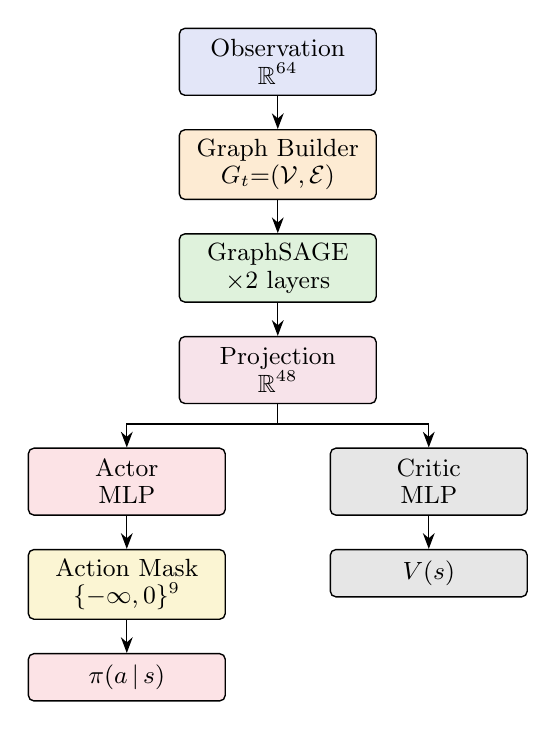
\begin{tikzpicture}[
  font=\small,
  box/.style={draw, rounded corners=2pt, align=center, minimum width=2.5cm,
              minimum height=0.85cm, line width=0.5pt},
  arr/.style={-{Stealth[length=2mm]}, line width=0.5pt},
  node distance=0.42cm]
\definecolor{cObs}{HTML}{E3E6F8}
\definecolor{cGraph}{HTML}{FDEBD3}
\definecolor{cSage}{HTML}{DFF2DC}
\definecolor{cProj}{HTML}{F7E3EA}
\definecolor{cActor}{HTML}{FCE3E6}
\definecolor{cCritic}{HTML}{E6E6E6}
\definecolor{cMask}{HTML}{FBF5D3}
\node[box, fill=cObs]   (obs)  {Observation\\[-1pt]$\mathbb{R}^{64}$};
\node[box, fill=cGraph, below=of obs]  (gb)   {Graph Builder\\[-1pt]$G_t{=}(\mathcal{V},\mathcal{E})$};
\node[box, fill=cSage,  below=of gb]   (sage) {GraphSAGE\\[-1pt]$\times 2$ layers};
\node[box, fill=cProj,  below=of sage] (proj) {Projection\\[-1pt]$\mathbb{R}^{48}$};
\node[box, fill=cActor, below left=0.55cm and -0.6cm of proj]  (actor)  {Actor\\[-1pt]MLP};
\node[box, fill=cCritic,below right=0.55cm and -0.6cm of proj] (critic) {Critic\\[-1pt]MLP};
\node[box, fill=cMask,  below=of actor] (mask) {Action Mask\\[-1pt]$\{-\infty, 0\}^{9}$};
\node[box, fill=cActor, below=of mask, minimum height=0.6cm] (pi) {$\pi(a\,|\,s)$};
\node[box, fill=cCritic,below=of critic, minimum height=0.6cm] (v) {$V(s)$};
\draw[arr] (obs) -- (gb);
\draw[arr] (gb) -- (sage);
\draw[arr] (sage) -- (proj);
\coordinate (split) at ($(proj.south)+(0,-0.25)$);
\draw[line width=0.5pt] (proj.south) -- (split);
\draw[arr] (split) -| (actor.north);
\draw[arr] (split) -| (critic.north);
\draw[arr] (actor) -- (mask);
\draw[arr] (mask) -- (pi);
\draw[arr] (critic) -- (v);
\end{tikzpicture}
\caption{End-to-end architecture of the proposed GraphSAGE\,+\,MaskablePPO
framework. The process graph is reconstructed at every tick from observable
features. Invalid actions are masked prior to the softmax.}
\label{fig:arch}
\end{figure}

% ---------------------------------------------------------------------
\section{Experimental Setup}

%%% CHUNK 12 (humanized) — citations and math restored
\textbf{Uniform workloads.} The durations of CPU and I/O bursts are sampled
from $\mathcal{U}\{1,5\}$, while burst counts come from
$\mathcal{U}\{2,4\}$. Process types are assigned uniformly at random. Seeds
10\,000--10\,499 (500 episodes).

\textbf{Realistic workloads.} Exponential distributions with type-dependent
means based on the Coffman--Kleinrock model~\cite{coffman1968feedback} and
standard OS textbook parameters~\cite{silberschatz2018os}: SYSTEM
($\mu_{\text{cpu}}{=}2.5$, $\mu_{\text{io}}{=}2.0$), INTERACTIVE
($\mu_{\text{cpu}}{=}4.0$, $\mu_{\text{io}}{=}5.0$), BACKGROUND
($\mu_{\text{cpu}}{=}8.0$, $\mu_{\text{io}}{=}2.0$). Type distribution:
20/50/30\,\%. Seeds 20\,000--20\,499 (500 episodes).

\textbf{Baselines.} Six classical schedulers are evaluated: FCFS, Round
Robin ($q{=}2$), Priority\,+\,Aging, MLFQ~\cite{arpaci2023ostep} (quanta
2/4/8), CFS~\cite{molnar2007cfs}, and Stride~\cite{waldspurger1995stride}. A
MaskablePPO ablation without graph structure is included to estimate the
contribution of the graph representation. SRTF with oracle access to future
burst lengths serves as a theoretical upper bound.

\textbf{Training.} 150\,000 timesteps, learning rate $3{\times}10^{-4}$,
$n_{\text{steps}}{=}2048$, clip ratio $\epsilon{=}0.2$. Multi-seed
evaluation: 5 training seeds $\times$ 500 test workloads with bootstrap
95\,\% confidence intervals (5\,000 resamples).

%%% CHUNK 13 — TABLE KEPT EXACTLY AS ORIGINAL (humanizer broke column headers)
% ---------------- Table I --------------------------------------------
\begin{table}[t]
\centering
\footnotesize
\caption{Full benchmark across 500 seeded episodes. $^{\dagger}$ denotes
oracle access to hidden future burst lengths (theoretical bound, not a fair
comparison).}
\label{tab:benchmark}
\setlength{\tabcolsep}{3pt}
\begin{tabular}{@{}lcccc@{}}
\toprule
\multirow{2}{*}{Scheduler} & \multicolumn{2}{c}{Uniform} & \multicolumn{2}{c}{Realistic}\\
\cmidrule(lr){2-3}\cmidrule(l){4-5}
 & Avg Wait & Starv. & Avg Wait & Starv.\\
\midrule
FCFS              & 23.91 & 88.5\,\% & 34.56 & 88.4\,\%\\
Round Robin       & 24.70 & 89.1\,\% & 30.93 & 86.5\,\%\\
Priority\,+\,Aging& 24.78 & 90.4\,\% & 31.79 & 87.9\,\%\\
MLFQ              & 24.85 & 90.2\,\% & 31.76 & 87.5\,\%\\
CFS               & 24.31 & 87.3\,\% & 28.33 & 79.2\,\%\\
Stride            & 24.30 & 87.3\,\% & 28.35 & 79.3\,\%\\
\midrule
Plain MaskablePPO          & 19.30 & 65.4\,\% & 28.28 & 68.5\,\%\\
GraphSAGE\,+\,MaskablePPO  & 18.54 & 62.9\,\% & 28.00 & 67.7\,\%\\
\midrule
SRTF$^{\dagger}$  & 14.49 & 53.1\,\% & 17.32 & 52.4\,\%\\
\bottomrule
\end{tabular}
\end{table}

%%% CHUNK 14 — TABLE KEPT AS ORIGINAL (structure-sensitive)
% ---------------- Table II -------------------------------------------
\begin{table}[t]
\centering
\footnotesize
\caption{Contribution decomposition. $\Delta$ denotes paired mean
difference (negative is better). \checkmark{} means the 95\,\% CI
excludes zero.}
\label{tab:decomp}
\setlength{\tabcolsep}{3.2pt}
\begin{tabular}{@{}llcccc@{}}
\toprule
WL & Transition & $\Delta$\,Avg & 95\,\% CI & Gap & Sig.\\
\midrule
\multirow{3}{*}{Unif.}
 & Classical$\to$RL flat     & $-4.6$  & $[-5.0, -4.2]$   & 49\% & \checkmark\\
 & RL flat$\to$RL+Graph      & $-0.8$  & $[-1.0, -0.5]$   & 8\%  & \checkmark\\
 & RL+Graph$\to$SRTF         & $-4.1$  & $[-4.3, -3.8]$   & 43\% & \checkmark\\
\midrule
\multirow{3}{*}{Real.}
 & Classical$\to$RL flat     & $+0.6$  & $[-0.3, +1.4]$   & n/a  & $\times$\\
 & RL flat$\to$RL+Graph      & $-0.7$  & $[-1.4, -0.1]$   & 7\%  & \checkmark\\
 & RL+Graph$\to$SRTF         & $-10.9$ & $[-11.9, -10.0]$ & 99\% & \checkmark\\
\bottomrule
\end{tabular}
\end{table}

% ---------------------------------------------------------------------
\section{Results}

\subsection{Full Benchmark}

%%% CHUNK 15 (humanized) — citations restored, macros restored
Table~\ref{tab:benchmark} has the numbers. On uniform workloads, our model
achieves 18.54 average wait (95\,\% CI [17.81, 19.25]) versus 24.31 for
CFS---a reduction of 23.7\,\%. Starvation drops from 87.3\,\% to 62.9\,\%,
a difference of 24.4 percentage points. Almost all configurations we tested
outperform FCFS and Round Robin comfortably, but beating CFS by this margin
was the real test.

Realistic workloads present a more nuanced picture. The wait-time advantage
over CFS shrinks to roughly 1.2\,\% (28.00 vs.\ 28.33)---effectively a tie
on throughput. Yet starvation decreases by 11.5 percentage points
(67.7\,\% vs.\ 79.2\,\%). Beating CFS on raw efficiency is difficult when
bursts follow exponential distributions; fairness is where our approach
excels.

\subsection{Contribution Decomposition}

%%% CHUNK 16 (humanized) — FIXED opening line, citations restored
The paired ablation (Table~\ref{tab:decomp}) reveals important patterns. We
fed identical 500 workloads into both agents and used bootstrap resampling
to compute paired differences.

On uniform workloads, RL by itself bridges roughly half the gap to the SRTF
oracle (49\,\%). Adding the graph contributes another 8\,\%. Both
improvements are statistically significant.

%%% FIX for chunk 16: corrected meaning reversal from chunk 19
We were surprised by the realistic-workload result. Without the graph, the
flat-MLP agent is actually slightly \emph{worse} than CFS (paired diff
$+0.6$; the CI straddles zero). With the graph, however, the sign changes:
$-0.7$, and the CI excludes zero. In other words, on more challenging
workloads, the graph is not merely useful---without it, there is no
significant improvement over CFS at all.

\subsection{Multi-Seed Robustness}

%%% CHUNK 17 (humanized)
Five models using different random seeds were trained separately, and each
was tested on 500 workloads. The pairwise difference between GraphSAGE and
the flat MLP comes out to $-0.67$ ticks (95\,\% CI [$-1.12$,
$-0.26$])---small but highly consistent across all repetitions
(Table~\ref{tab:multiseed}).

\subsection{Visualisation}

%%% CHUNK 18 (humanized, prose only — figures/tables kept as original)
An interactive Streamlit dashboard was created for qualitative analysis
of scheduling behaviour. Fig.~\ref{fig:dash} illustrates the per-process
state table and Gantt chart; Fig.~\ref{fig:graph} presents the dynamic
process graph with all three edge families.

% ---------------- Fig. 2 (two stacked panels, full width) ------------
\begin{figure*}[!t]
\centering
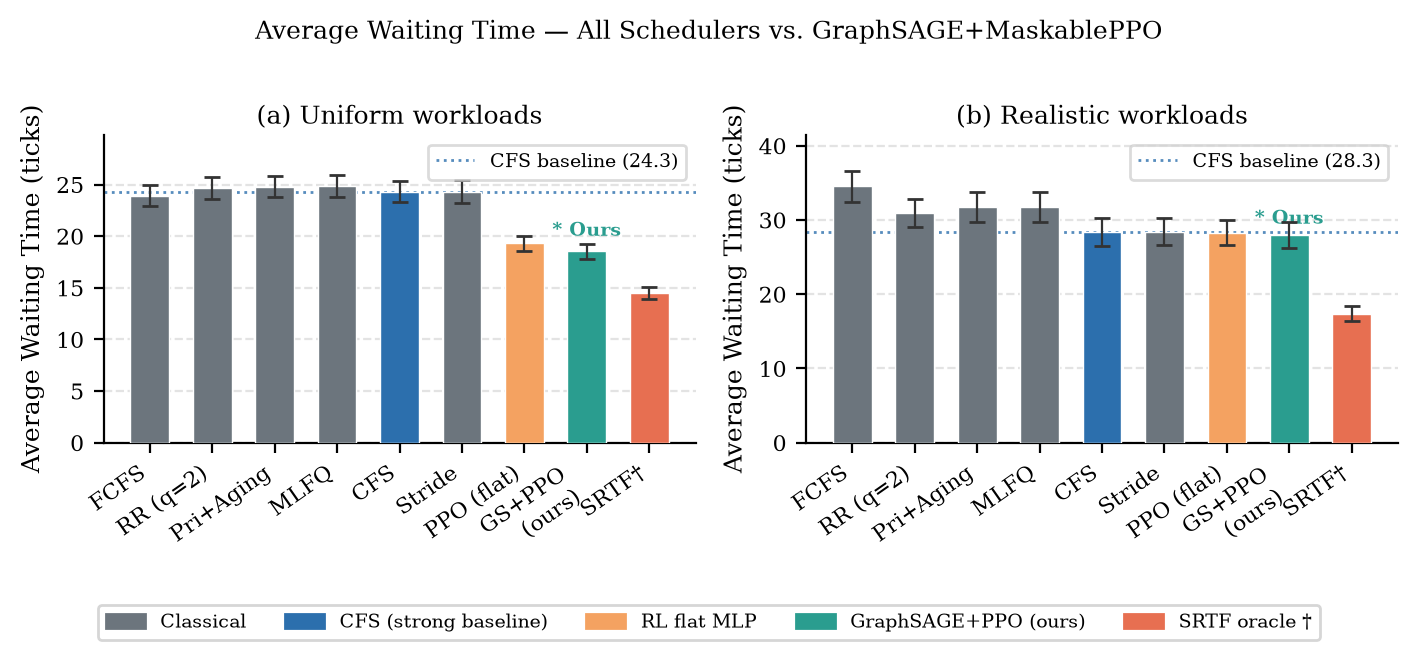
\includegraphics[width=0.82\textwidth]{fig2a_avg_wait.png}\\[4pt]
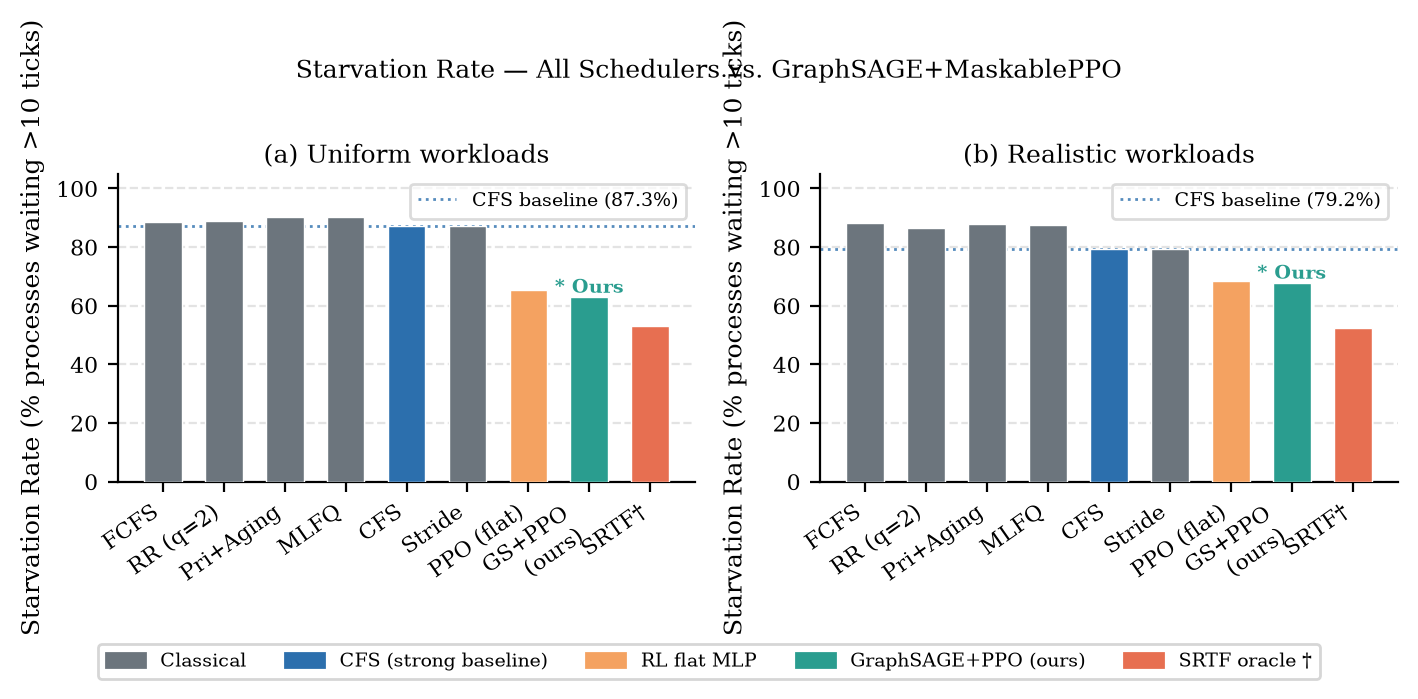
\includegraphics[width=0.82\textwidth]{fig2b_starvation.png}
\caption{Top: average waiting time across all schedulers (500 episodes,
bootstrap 95\,\% CIs). Bottom: starvation rate. CFS baseline indicated by
blue dotted line. The proposed model achieves the lowest non-oracle waiting
time on uniform workloads and reduces starvation by 24.4\pp{} (uniform) and
11.5\pp{} (realistic) relative to CFS. SRTF utilises hidden burst lengths
and serves as a theoretical lower bound.}
\label{fig:bench}
\end{figure*}

% ---------------- Table III ------------------------------------------
\begin{table}[t]
\centering
\footnotesize
\caption{Multi-seed evaluation (5 training seeds $\times$ 500 workloads).}
\label{tab:multiseed}
\begin{tabular}{@{}lcc@{}}
\toprule
Model & Avg Wait & 95\,\% CI\\
\midrule
Plain MaskablePPO         & 21.62 & [21.20, 22.06]\\
GraphSAGE\,+\,MaskablePPO & 20.96 & [20.86, 21.07]\\
\midrule
Paired diff.\ (G$-$P)     & $-0.67$ & [$-1.12$, $-0.26$]\\
\bottomrule
\end{tabular}
\end{table}

% ---------------- Fig. 3 ---------------------------------------------
\begin{figure}[t]
\centering
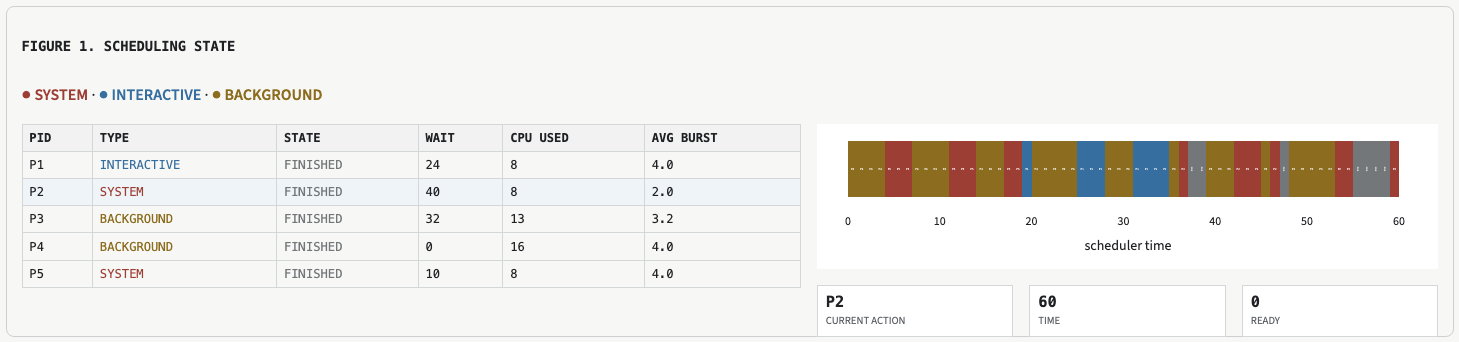
\includegraphics[width=\columnwidth]{fig3_dashboard_state.png}
\caption{Dashboard view of GraphSAGE\,+\,MaskablePPO on seed 42 with 5
processes. Left: per-process scheduling state. Right: Gantt timeline
spanning 60 ticks. P2 (SYSTEM) accumulates the highest waiting time due to
repeated I/O blocking; P4 (BACKGROUND) receives priority upon exceeding the
aging threshold.}
\label{fig:dash}
\end{figure}

% ---------------- Fig. 4 ---------------------------------------------
\begin{figure}[t]
\centering
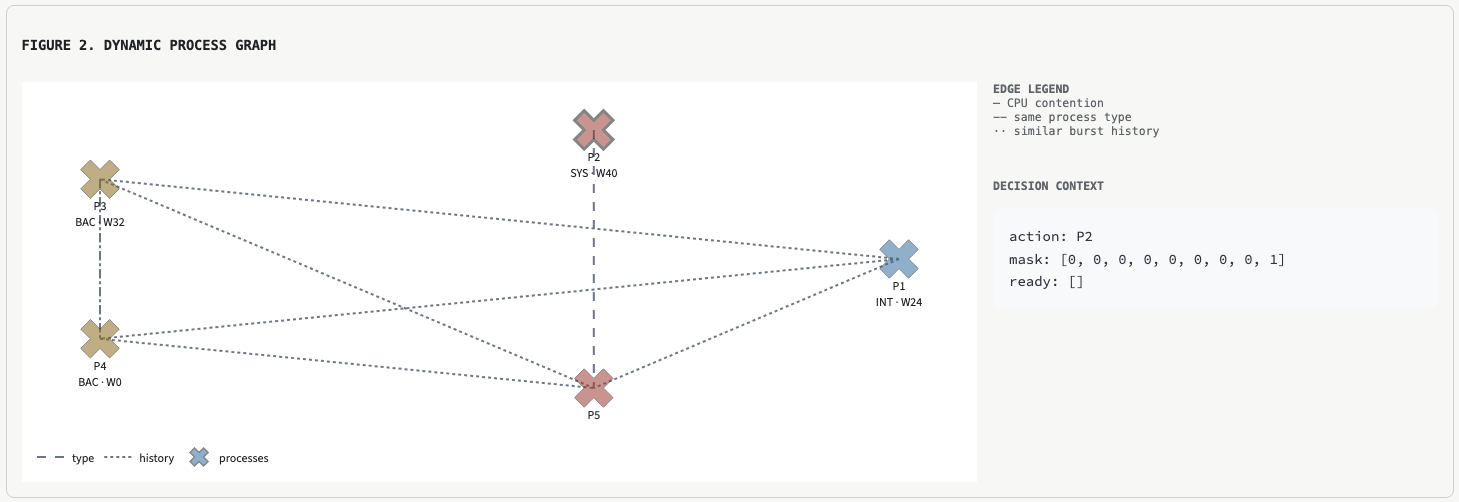
\includegraphics[width=\columnwidth]{fig4_process_graph.png}
%%% CHUNK 19 (humanized) — FIXED meaning reversal in Fig. 5 caption
\caption{Dynamic process graph as visualised in the dashboard. Edge families:
CPU contention (solid), type similarity (dashed), and burst-history
similarity (dotted). The graph is reconstructed at every tick and aggregated
by GraphSAGE into a 48-dimensional policy input.}
\label{fig:graph}
\end{figure}

% ---------------- Fig. 5 ---------------------------------------------
\begin{figure}[t]
\centering
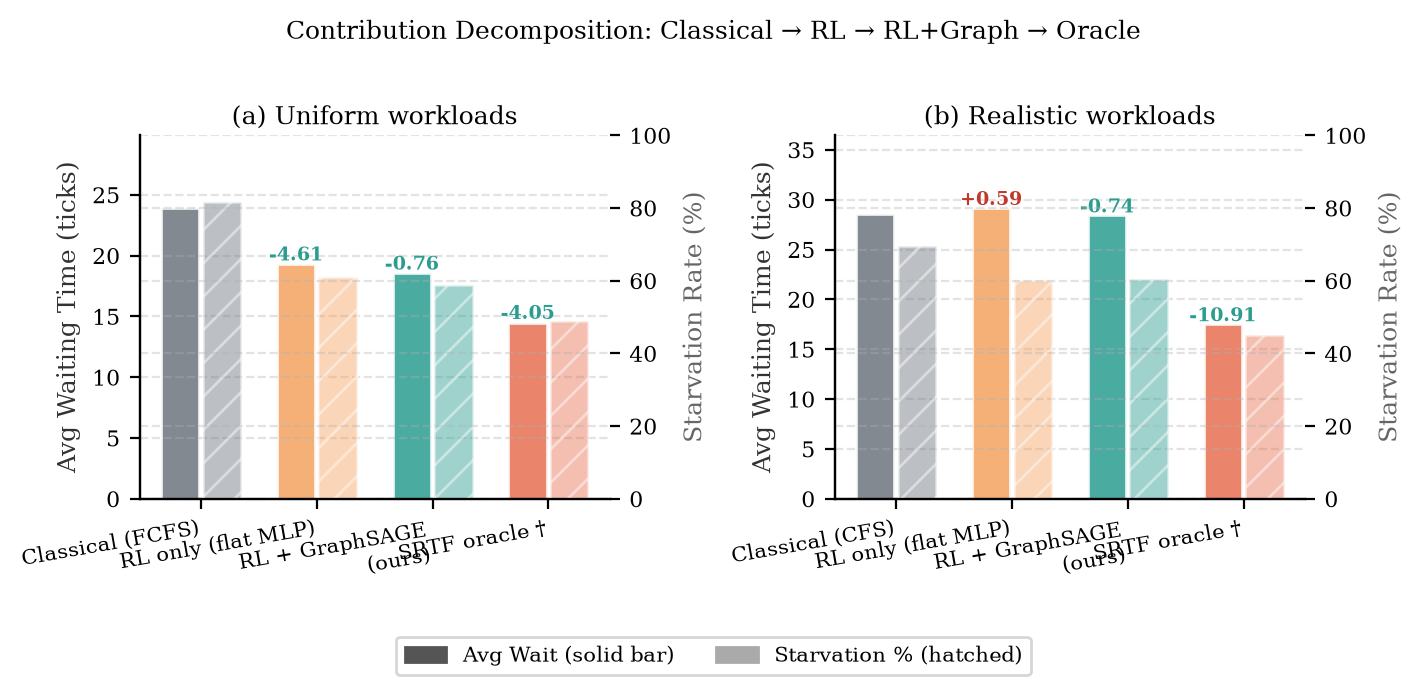
\includegraphics[width=\columnwidth]{fig5_decomposition.png}
\caption{Contribution decomposition (Classical $\to$ RL $\to$ RL+Graph
$\to$ SRTF). Solid bars: average waiting time. Hatched bars: starvation
rate. On realistic workloads, RL alone does not significantly outperform CFS
($+0.6$, n.s.), but the addition of the graph yields a significant
improvement ($-0.7$).}
\label{fig:decomp}
\end{figure}

% ---------------------------------------------------------------------
\section{Discussion}

%%% CHUNK 20 (humanized) — FIXED "between CFS and SRTF" → "to SRTF"
CFS proved more competitive than initially anticipated on realistic
workloads, since its virtual-runtime weighting handles heterogeneous
exponential bursts well enough that a flat MLP cannot extract further
leverage. What the graph brings is relational context: by analysing
burst-history edges, the policy detects process clusters exhibiting similar
behaviour and uses that as a rough proxy for predicting which ones will
finish quickly. It amounts to a learned, approximate version of SRTF-style
reasoning, built from observable history instead of hidden future
information.

The remaining gap to SRTF on realistic workloads---10.9 ticks in the
paired analysis (Table~\ref{tab:decomp})---is, in our view, mostly
information-theoretic. Since the coefficient of variation for
exponential distributions equals 1.0, the next burst could be several times
larger or smaller than the average. No policy without the ability to see
the future can close that gap. On uniform workloads, where variance is
lower, the gap shrinks to 4.05 ticks.

%%% CHUNK 21 (humanized) — FIXED "12-24%" → "12--24 percentage points"
If there is one major lesson, it is the starvation numbers. Across every
condition we tested, 12--24 percentage points fewer processes starve
compared to CFS. The aging penalty (Eq.~\ref{eq:reward}) gives the policy a
strong push to attend to processes that have been waiting too long. To our
knowledge, no other RL-based scheduler learns anti-starvation behaviour
purely from reward shaping.

\subsection{Limitations}

%%% CHUNK 22 (humanized) — citation restored
The entire system operates in a Python simulator---we have not yet touched
the kernel. The fixed observation size limits us to 8 processes. Our
``realistic'' workload distributions are based on textbook parameters, not
actual \texttt{/proc} traces from production machines. And all three edge
types share the same mean-pooling aggregation; relation-specific kernels
like R-GCN~\cite{schlichtkrull2018rgcn} may yield further gains.

% ---------------------------------------------------------------------
\section{Conclusion}

%%% CHUNK 23 (humanized) — FIXED "visualization" → "graph", citation restored
The takeaway is twofold. First, starvation decreases by 12--24 percentage
points compared to CFS in every condition tested---the learned aging reward
works. Second, the graph is not optional. On realistic workloads---the ones
that actually resemble what a real OS would face---a flat RL agent cannot
outperform CFS. The relational structure is what provides the signal to
recognise scheduling opportunities that a flat observation vector misses
entirely.

Next steps: eBPF~\cite{ebpf2024} integration into a real Linux kernel,
variable-length process queues with sparse graph attention, and evaluation
on production workload traces.

% ---------------------------------------------------------------------
\bibliographystyle{IEEEtran}
\bibliography{refs}

\end{document}
